%=================================================================
%  15.C51 --- Project #1 (Proprietary Trading Track)
%
%  Mean-Reversion vs. Momentum Across Horizons:
%  A Data-Source-Matched Comparison on the Dow Jones 30
%
%  Data:  CRSP Daily  +  WRDS Intraday Indicators (iid_ms)
%         +  TAQ Millisecond (stretch)
%
%  Guide v3 --- LEAN & FOCUSED
%  The study is a comparison across horizons; every design
%  choice is subordinate to making that comparison clean.
%=================================================================

\documentclass[11pt,letterpaper]{article}

% ----------- PACKAGES --------------------------------------------
\usepackage[margin=1in]{geometry}
\usepackage{amsmath,amssymb,mathtools}
\usepackage{graphicx}
\usepackage{booktabs,array,tabularx,longtable}
\usepackage{float}
\usepackage{caption}
\usepackage{hyperref}
\usepackage{xcolor}
\usepackage{enumitem}
\usepackage{tikz}
\usepackage{pgfplots}
\pgfplotsset{compat=1.18}
\usepackage{listings}
\usepackage{fancyhdr}
\usepackage{titlesec}
\usepackage{parskip}
\usepackage{microtype}
\usetikzlibrary{shapes.geometric, positioning}

% ----------- COLORS ----------------------------------------------
\definecolor{mitred}{RGB}{163,31,52}
\definecolor{accent}{RGB}{20,80,140}
\definecolor{meanrev}{RGB}{50,120,90}
\definecolor{momcol}{RGB}{190,80,50}
\definecolor{softgray}{RGB}{245,245,245}
\definecolor{notecol}{RGB}{50,90,130}

% ----------- HYPERREF --------------------------------------------
\hypersetup{
  colorlinks=true,
  linkcolor=accent,
  urlcolor=accent,
  citecolor=accent
}

% ----------- PAGE STYLE ------------------------------------------
\pagestyle{fancy}
\fancyhf{}
\fancyhead[L]{\small 15.C51 Project 1}
\fancyhead[R]{\small Horizon Comparison Guide}
\fancyfoot[C]{\thepage}
\renewcommand{\headrulewidth}{0.4pt}

% ----------- SECTION STYLING -------------------------------------
\titleformat{\section}
  {\color{mitred}\Large\bfseries}{\thesection}{0.6em}{}
\titleformat{\subsection}
  {\color{accent}\large\bfseries}{\thesubsection}{0.5em}{}

% ----------- CUSTOM BOX ------------------------------------------
\newenvironment{keybox}[1][Key Point]
  {\begin{center}\begin{minipage}{0.95\linewidth}\vspace{2pt}
   \rule{\linewidth}{0.5pt}\par\textbf{#1.}\par\vspace{-2pt}}
  {\par\rule{\linewidth}{0.5pt}\end{minipage}\end{center}}

% ----------- LISTINGS -------------------------------------------
\lstset{
  basicstyle=\ttfamily\small,
  backgroundcolor=\color{softgray},
  frame=single,
  rulecolor=\color{black!30},
  breaklines=true,
  keywordstyle=\color{accent}\bfseries,
  commentstyle=\color{gray}\itshape,
  showstringspaces=false,
  numbers=left,
  numberstyle=\tiny\color{gray}
}

% ----------- MATH SHORTCUTS -------------------------------------
\newcommand{\E}{\mathbb{E}}
\newcommand{\Var}{\mathrm{Var}}
\newcommand{\Cov}{\mathrm{Cov}}
\newcommand{\Corr}{\mathrm{Corr}}
\newcommand{\sign}{\operatorname{sign}}
\newcommand{\VR}{\mathrm{VR}}

% ----------- TITLE -----------------------------------------------
\title{\vspace{-1.5cm}\color{mitred}\textbf{Mean-Reversion vs. Momentum Across Horizons}\\[0.3em]
\Large\color{accent}A Data-Source-Matched Comparison on the Dow Jones 30 \\[0.6em]
\large\color{black}\normalfont Project Guide v3 --- 15.C51, Spring 2026}
\author{Modeling with Machine Learning: Financial Technology\\Project \#1 --- Proprietary Trading Track}
\date{\today}

\begin{document}
\maketitle
\thispagestyle{empty}

\begin{abstract}
\noindent We compare two strategy families---\textbf{mean-reversion} and \textbf{momentum}---across six return horizons spanning nine orders of magnitude in time, from minutes to a year. The three datasets at our disposal each have a natural horizon domain: \textbf{TAQ Millisecond} for minutes, \textbf{WRDS Intraday Indicators} (\texttt{iid\_ms}) for the intraday/daily boundary, and \textbf{CRSP Daily} for days to years. By applying a \emph{single, uniform} strategy specification at every horizon, the study turns into a clean A/B/\dots{} comparison: we read off the horizon at which each phenomenon dominates, and we let that reading pick the two strategies we put into the ICM. This guide specifies the universe, the unified methodology, the six horizons, the expected outcomes, and the final deliverable.
\end{abstract}

\tableofcontents
\newpage

%=================================================================
\section{Executive Summary}\label{sec:summary}
%=================================================================

\subsection{One-paragraph framing}

Project~1 asks us to build a mean-reversion strategy and a momentum strategy on DJ30 using 10 years of price data and to deliver an Investment Committee Memorandum (ICM). We keep the deliverable and enrich the analysis with a \emph{single methodological move}: we run \emph{both} strategies at \emph{six different horizons}, each horizon naturally served by one of our three datasets (TAQ, \texttt{iid\_ms}, CRSP). The comparison is the study; the two strategies in the ICM are whichever horizon-specific best-performers emerge.

\subsection{Hypothesis}

Mean-reversion dominates at very short (microstructure) and medium (daily--monthly) horizons, while momentum dominates at intraday and intermediate (3--12 month) horizons. If our data confirm this pattern, we will select one winning mean-reversion horizon and one winning momentum horizon for the ICM.

\subsection{Deliverable}

One ICM containing: (i)~the two chosen strategies and their full specification; (ii)~the horizon-comparison table as the headline empirical evidence; (iii)~statistical properties, profit/loss conditions, and historical performance for each chosen strategy.

%=================================================================
\section{The Research Question}\label{sec:question}
%=================================================================

\subsection{Why comparison across horizons is the project}

The first-order autocorrelation of individual-stock returns, $\rho_1(h) = \Corr(r_{t,h}, r_{t-h,h})$, changes sign multiple times as we vary the return horizon $h$. Negative $\rho_1(h)$ implies mean-reverting returns over that horizon; positive $\rho_1(h)$ implies trending returns. A portfolio that \emph{trades against} the observed autocorrelation sign at horizon $h$ is a bet on $\rho_1(h)$ being of the expected sign out-of-sample.

This single framing unifies the two strategies the assignment asks about: they are the \emph{same} portfolio construction applied at different horizons, with opposite signs.

\subsection{The central question}

\begin{keybox}[Research question]
For DJ30 stocks over 2016--2026, at which horizons is the cross-sectional ranking by past return a \emph{negative} (reversal) predictor of next-period return, and at which horizons is it a \emph{positive} (momentum) predictor? What net-of-cost Sharpe ratio does a simple long--short portfolio achieve at each horizon?
\end{keybox}

\subsection{What we are not doing}

To keep the study focused, we deliberately \emph{exclude}:
\begin{itemize}[leftmargin=*]
  \item Multi-factor or blended strategies (no STR $\times$ MHM combinations).
  \item Machine-learning models beyond a single benchmark specification check.
  \item Regime-conditional signals (we report regime-split results but do not trade them).
  \item Options, ETF arbitrage, or cross-asset constructions.
\end{itemize}
Every design choice serves the comparison.

%=================================================================
\section{The Six Horizons}\label{sec:horizons}
%=================================================================

\subsection{Horizons matched to data sources}

\begin{table}[H]
\centering
\small
\renewcommand{\arraystretch}{1.3}
\begin{tabularx}{\linewidth}{@{}l l l X@{}}
\toprule
\textbf{Label} & \textbf{Horizon $h$} & \textbf{Data source} & \textbf{Expected phenomenon and reference}\\
\midrule
H1 & $5$\,min -- $30$\,min  & TAQ (stretch)       & Intraday momentum / microstructure reversal (Gao et al.\ 2018; Roll 1984)\\
H2 & $1$\,day (O2C + overnight split) & \texttt{iid\_ms}    & Intraday momentum persistence (Gao, Han, Li, Zhou 2018)\\
H3 & $1$\,day (close-to-close) & CRSP daily       & Short-term reversal (Lehmann 1990)\\
H4 & $5$\,days (weekly)     & CRSP daily          & Short-term reversal (Lo \& MacKinlay 1990)\\
H5 & $21$\,days (monthly)   & CRSP daily          & One-month reversal (Jegadeesh 1990)\\
H6 & $126$\,days (6~months) & CRSP daily          & Intermediate momentum (Jegadeesh \& Titman 1993)\\
\bottomrule
\end{tabularx}
\caption{The six horizons we study, each naturally served by one dataset. The expected phenomenon is the sign the classical literature predicts. Our central empirical question is whether those signs persist in DJ30 over 2016--2026.}
\label{tab:horizons}
\end{table}

\subsection{The picture we will fill in}

\begin{figure}[H]
\centering
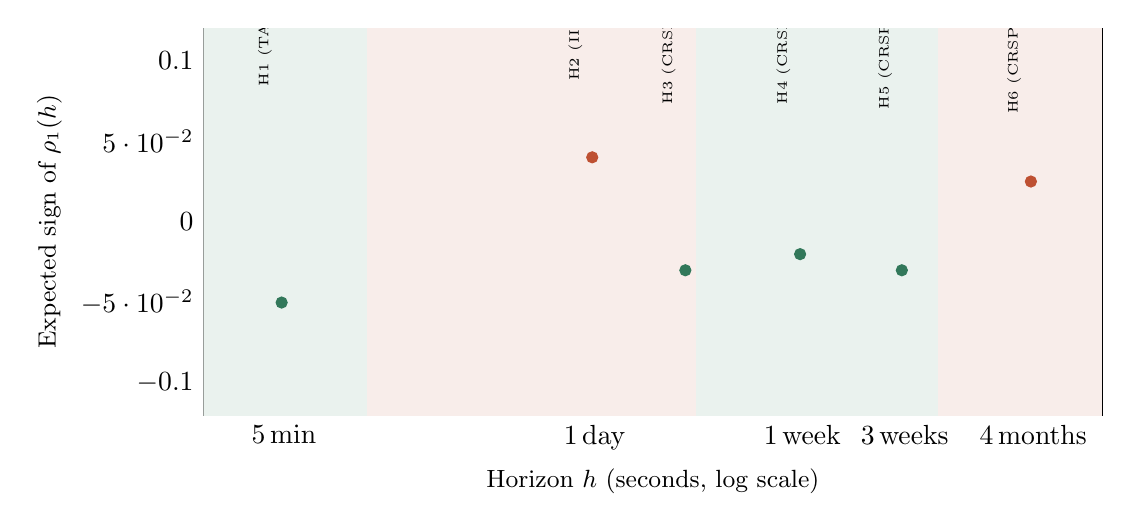
\begin{tikzpicture}
\begin{axis}[
    width=13cm, height=6.5cm,
    xmode=log,
    xmin=1e2, xmax=3e7,
    ymin=-0.12, ymax=0.12,
    xlabel={Horizon $h$ (seconds, log scale)},
    ylabel={Expected sign of $\rho_1(h)$},
    ytick={-0.1,-0.05,0,0.05,0.1},
    xtick={300,23400,432000,1814400,1.1e7},
    xticklabels={\,5\,min,\,1\,day,\,1\,week,\,3\,weeks,\,4\,months},
    xlabel style={font=\small},
    ylabel style={font=\small},
    grid=both,
    grid style={dashed, gray!30},
]
\addplot[black, thick, dashed, domain=1e2:3e7] {0};

% Shaded backgrounds
\fill[meanrev!10] (axis cs:1e2,-0.12) rectangle (axis cs:1000,0.12);
\fill[momcol!10]  (axis cs:1000,-0.12) rectangle (axis cs:1e5,0.12);
\fill[meanrev!10] (axis cs:1e5,-0.12) rectangle (axis cs:3e6,0.12);
\fill[momcol!10]  (axis cs:3e6,-0.12) rectangle (axis cs:3e7,0.12);

% Horizon markers
\node[font=\tiny, rotate=90, anchor=south] at (axis cs:300,0.11) {H1 (TAQ)};
\node[font=\tiny, rotate=90, anchor=south] at (axis cs:23400,0.11) {H2 (IID)};
\node[font=\tiny, rotate=90, anchor=south] at (axis cs:86400,0.11) {H3 (CRSP 1d)};
\node[font=\tiny, rotate=90, anchor=south] at (axis cs:432000,0.11) {H4 (CRSP 5d)};
\node[font=\tiny, rotate=90, anchor=south] at (axis cs:1.8e6,0.11) {H5 (CRSP 21d)};
\node[font=\tiny, rotate=90, anchor=south] at (axis cs:1.1e7,0.11) {H6 (CRSP 126d)};

% Literature marks
\addplot[only marks, mark=*, mark size=2pt, color=meanrev]
coordinates {(300,-0.05)};
\addplot[only marks, mark=*, mark size=2pt, color=momcol]
coordinates {(23400,0.04)};
\addplot[only marks, mark=*, mark size=2pt, color=meanrev]
coordinates {(86400,-0.03)};
\addplot[only marks, mark=*, mark size=2pt, color=meanrev]
coordinates {(432000,-0.02)};
\addplot[only marks, mark=*, mark size=2pt, color=meanrev]
coordinates {(1.8e6,-0.03)};
\addplot[only marks, mark=*, mark size=2pt, color=momcol]
coordinates {(1.1e7,0.025)};
\end{axis}
\end{tikzpicture}
\caption{The literature-predicted sign pattern we will test. Green points indicate the three reversal horizons (H1 under microstructure, H3, H4, H5); red points indicate the two momentum horizons (H2 intraday, H6 intermediate). Our empirical study replaces each dot with an actual estimate from DJ30 2016--2026.}
\label{fig:hypothesis}
\end{figure}

\subsection{What success looks like}

A successful comparison produces the table in Section~\ref{sec:deliverable} with six rows and clear column values. We do \emph{not} require every expected sign to be confirmed; a horizon where the classical sign \emph{fails} in our DJ30 window is itself a finding worth documenting.

%=================================================================
\section{Unified Methodology}\label{sec:method}
%=================================================================

This section specifies, once, a methodology that is \emph{applied identically} at every horizon. Uniformity is what makes the comparison meaningful.

\subsection{Universe: point-in-time DJ30}

For each date $t$ in our 2016--2026 window, let $U_t \subseteq \{1,\dots,38\}$ be the set of stocks that are index members as of that date's close. The DJ30 has changed members several times in our window (notable events: GE $\to$ WBA in Jun~2018; UTX $\to$ RTX in Apr~2020; the PFE/XOM/RTX $\to$ CRM/AMGN/HON rebalance in Aug~2020; WBA/DOW/INTC $\to$ AMZN/SHW/NVDA in 2024); using today's membership is survivorship bias. Build $U_t$ from the S\&P Dow Jones Indices press-release history and assert $|U_t|=30$ on every trading date.

\subsection{Signal: past-horizon return}

For each stock $i\in U_t$ and each horizon $h\in\{\text{H1},\dots,\text{H6}\}$ we compute the \emph{past $h$-period return}:
\begin{equation}
s^{(h)}_{i,t} = \frac{P_{i,t}}{P_{i,t-h}} - 1,
\label{eq:signal}
\end{equation}
using total returns (dividends reinvested) from the appropriate data source.

\subsection{Portfolio construction: tercile long--short}

At the end of each period of length~$h$, sort $U_t$ by $s^{(h)}_{i,t}$. Form two portfolios:

\begin{itemize}[leftmargin=*]
  \item \textbf{Momentum portfolio (MOM-$h$)}: long the top tercile of $s^{(h)}$, short the bottom tercile.
  \item \textbf{Mean-reversion portfolio (REV-$h$)}: long the bottom tercile of $s^{(h)}$, short the top tercile.
\end{itemize}

Both are equal-weighted within each leg, dollar-neutral across legs, and held for exactly one horizon period before rebalancing. With $|U_t|=30$ the terciles contain 10 names each; $t$-statistics will scale accordingly.

Formally, let $\mathrm{rk}_{i,t}$ be the rank of $s^{(h)}_{i,t}$ in $U_t$, with $\mathrm{rk}\in\{1,\dots,30\}$. Define tercile membership:
\begin{equation}
w^{\text{MOM}}_{i,t+h} = \frac{1}{10}\bigl[\mathbf{1}(\mathrm{rk}_{i,t}>20) - \mathbf{1}(\mathrm{rk}_{i,t}\le 10)\bigr],
\end{equation}
and $w^{\text{REV}}_{i,t+h} = -w^{\text{MOM}}_{i,t+h}$. The two portfolios are exact mirror images. Gross leverage is one ($\sum_i |w_i| = 1$).

\begin{keybox}[Why so simple?]
A classical, transparent portfolio construction makes the horizon comparison clean. An ML-enhanced specification is reported as a robustness check (Section~\ref{sec:robust}), not as the headline.
\end{keybox}

\subsection{Horizon-specific adjustments}

Two horizons need small adjustments for data availability:

\begin{itemize}[leftmargin=*]
  \item \textbf{H1 (TAQ):} the universe is rebuilt from TAQ 5-min bars; rebalance cadence is every 30~min during regular trading hours. The tercile construction is the same.
  \item \textbf{H2 (\texttt{iid\_ms}):} the signal is the \emph{first-half-hour} return (9:30--10:00\,ET) of day~$t$, and the forward return is the \emph{rest-of-day} return (10:00--16:00\,ET) of the same day, following Gao, Han, Li, and Zhou (2018). This is a ``within-day'' horizon.
\end{itemize}

For the four CRSP horizons (H3--H6), the signal is past-$h$-day cumulative return and the forward return is the next $h$-day cumulative return.

\subsection{Transaction costs}

We apply a single, consistent cost model so that horizons can be compared on a like-for-like basis: a per-side cost of $c_h$ bps applied to turnover,
\begin{equation}
r^{\text{net}}_{p,t+h} = r^{\text{gross}}_{p,t+h} - c_h \cdot \text{turnover}_{t+h},
\end{equation}
where turnover is $\sum_i |w_{i,t+h} - w_{i,t}|$. The cost $c_h$ is calibrated to the typical effective spread at that horizon (see Table~\ref{tab:costs}):

\begin{table}[H]
\centering
\small
\begin{tabular}{@{}lcc@{}}
\toprule
\textbf{Horizon} & \textbf{Per-side cost $c_h$ (bps)} & \textbf{Rationale}\\
\midrule
H1 (intraday, TAQ 30\,min)      & 3.0 & ES + maker/taker fees at DJ30 ticker liquidity\\
H2 (intraday, \texttt{iid\_ms}) & 1.5 & One rebalance per day; trade at VWAP/TWAP\\
H3 (daily)                      & 1.5 & Same as H2; daily close execution\\
H4 (weekly)                     & 1.5 & Same\\
H5 (monthly)                    & 1.5 & Same\\
H6 (6-month)                    & 1.5 & Same\\
\bottomrule
\end{tabular}
\caption{Cost model. H1 pays a higher per-side cost because intraday execution crosses spreads at higher participation than VWAP-scheduled daily execution.}
\label{tab:costs}
\end{table}

\subsection{Performance metrics}

Every strategy at every horizon is reported with the same metrics:

\begin{enumerate}[leftmargin=*]
  \item Annualized return (gross \emph{and} net of cost).
  \item Annualized volatility.
  \item Annualized Sharpe ratio: $\text{SR} = \sqrt{a_h}\cdot \bar r/\hat\sigma$, where $a_h$ is the annualization factor (e.g., $a_{\text{H5}} = 12$ for monthly; $a_{\text{H3}} = 252$ for daily).
  \item Max drawdown.
  \item $t$-statistic of the mean net return against zero.
  \item Turnover per rebalance and annualized.
\end{enumerate}

\subsection{Inference across horizons}

The comparison across horizons is done on \textbf{Sharpe ratio} (scale-free) and \textbf{$t$-statistic} (which has the same null at every horizon). To assess joint significance we apply a Bonferroni correction over the 12 tests (6 horizons $\times$ 2 strategies): a single strategy's $t$ must exceed the Bonferroni-adjusted threshold $t^* = \Phi^{-1}(1-0.025/12) \approx 2.87$ to be called ``significant'' at the 5\% family-wise error rate.

%=================================================================
\section{Data Sources}\label{sec:data}
%=================================================================

\subsection{CRSP Daily (serves H3--H6)}

CRSP provides daily total returns, prices, shares outstanding, and adjustment factors for every U.S.-listed stock back to 1926. The relevant fields we use from \texttt{crsp.dsf}:

\begin{center}\small
\begin{tabular}{@{}lll@{}}
\toprule
\textbf{Field} & \textbf{Purpose} & \textbf{Quirks}\\
\midrule
\texttt{permno} & Stock identifier (stable across ticker changes) & Use permno, not ticker\\
\texttt{ret}    & Daily total return & Includes dividends and distributions\\
\texttt{prc}    & Closing price (negative = midquote used) & Take \texttt{abs(prc)}\\
\texttt{cfacpr} & Price adjustment factor & Divide raw price for adjusted price\\
\texttt{vol}    & Share volume & Multiply by price for dollar volume\\
\bottomrule
\end{tabular}
\end{center}

CRSP is canonical for H3--H6. Returns over longer horizons are constructed by compounding daily returns.

\subsection{WRDS Intraday Indicators \texttt{iid\_ms} (serves H2)}

\texttt{iid\_ms} is a \emph{daily panel} of pre-computed microstructure statistics derived from millisecond-stamped TAQ. Each row is a security-day; intraday resolution is encoded in column values, not in row cadence. Key fields for this project:

\begin{center}\small
\begin{tabular}{@{}ll@{}}
\toprule
\textbf{Field family} & \textbf{Use in this study}\\
\midrule
AM/PM return split (if present) & Direct H2 signal construction\\
Realized volatility (RV), bipower variation  & Risk weighting, jump-day flagging\\
Effective spread                             & Horizon-appropriate cost floor\\
Order imbalance, Amihud illiquidity          & Robustness conditioning\\
\bottomrule
\end{tabular}
\end{center}

\subsection{TAQ Millisecond (serves H1, stretch)}

TAQ contains every consolidated trade and NBBO quote at millisecond resolution. For H1 we aggregate trades into 30-minute bars for each DJ30 name and compute 30-minute returns. For 10 years $\times$ 30 names $\times$ $\sim$13 bars/day, the panel is $\sim$10~M rows---manageable in Parquet partitioned by year.

TAQ is a \emph{stretch} data source: if the pull proves operationally hard, we report H1 only via the microstructure literature without our own backtest, and the comparison table drops H1.

\subsection{Data flow}

\begin{figure}[H]
\centering
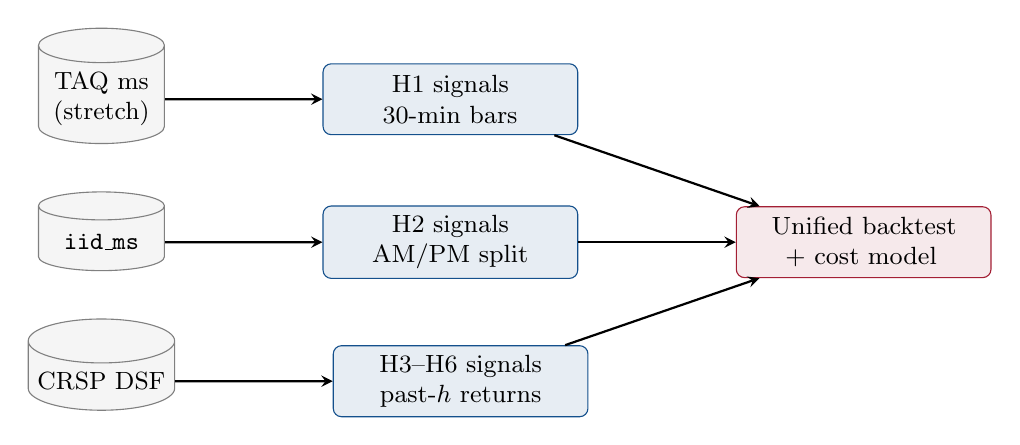
\begin{tikzpicture}[node distance=0.6cm and 1cm,
  db/.style={cylinder, shape border rotate=90, draw=black!50, aspect=0.3,
             minimum height=1cm, minimum width=1.6cm, fill=softgray, align=center, font=\small},
  box/.style={rectangle, draw=accent, rounded corners=3pt, minimum height=0.9cm,
              text width=3cm, align=center, fill=accent!10, font=\small},
  output/.style={rectangle, draw=mitred, rounded corners=3pt, minimum height=0.9cm,
              text width=3cm, align=center, fill=mitred!10, font=\small},
  arrow/.style={-stealth, thick}]

\node[db] (taq)  {TAQ ms\\(stretch)};
\node[db, below=of taq]  (iid)  {\texttt{iid\_ms}};
\node[db, below=of iid]  (crsp) {CRSP DSF};

\node[box, right=2cm of taq]  (b1) {H1 signals\\30-min bars};
\node[box, right=2cm of iid]  (b2) {H2 signals\\AM/PM split};
\node[box, right=2cm of crsp] (b3) {H3--H6 signals\\past-$h$ returns};

\node[output, right=2cm of b2] (bt) {Unified backtest\\+ cost model};

\draw[arrow] (taq)  -- (b1);
\draw[arrow] (iid)  -- (b2);
\draw[arrow] (crsp) -- (b3);
\draw[arrow] (b1) -- (bt);
\draw[arrow] (b2) -- (bt);
\draw[arrow] (b3) -- (bt);
\end{tikzpicture}
\caption{Each data source feeds the horizon it naturally serves. A single backtest loop with identical methodology consumes all six signal streams.}
\end{figure}

%=================================================================
\section{Horizon-by-Horizon Notes}\label{sec:notes}
%=================================================================

Brief context for each horizon: canonical reference, economic mechanism, and an implementation note.

\subsection{H1 --- 30-minute bars (TAQ)}

\textbf{Reference:} Roll (1984) for microstructure reversal; Gao et al.\ (2018) for intraday momentum. \textbf{Mechanism:} at 5--30 minute horizons, returns are a mixture of short-lived bid-ask bounce (reversal) and information-driven continuation (momentum). In large, liquid DJ30 names, we expect near-zero net autocorrelation, making H1 the \emph{hardest} horizon to profit at and a useful null. \textbf{Implementation:} 30-min TAQ bars, skip the first and last 15 minutes of each session (opening/closing auction effects).

\subsection{H2 --- Intraday first-half-hour $\to$ rest-of-day (\texttt{iid\_ms})}

\textbf{Reference:} Gao, Han, Li, Zhou (2018, JFE). \textbf{Mechanism:} the first-half-hour absorbs overnight information; the rest-of-day rides institutional rebalancing flows. They document significant positive $\beta$ in $r^{\text{rest}}_t = \alpha + \beta r^{\text{first-30}}_t + \epsilon$. \textbf{Implementation:} if \texttt{iid\_ms} provides AM/PM splits, use them directly; otherwise this horizon requires TAQ.

\subsection{H3 --- 1-day close-to-close (CRSP)}

\textbf{Reference:} Lehmann (1990, QJE). \textbf{Mechanism:} one-day reversal is compensation for liquidity provision: a name that fell sharply was absorbed by liquidity suppliers who are paid back the next day. \textbf{Caveat for DJ30:} large caps have weaker reversal than the CRSP-wide universe because they are already well-supplied with liquidity; expect modest $t$-statistics.

\subsection{H4 --- 5-day weekly (CRSP)}

\textbf{Reference:} Lo \& MacKinlay (1990, RFS). They decompose contrarian profits into own-autocovariance, cross-autocovariance (lead--lag), and common-factor terms, and find that lead--lag dominates in CRSP-wide panels. On DJ30, with no small-cap component, the lead--lag channel is weaker. \textbf{Implementation:} straightforward compounded 5-day returns.

\subsection{H5 --- 21-day monthly (CRSP)}

\textbf{Reference:} Jegadeesh (1990, J.~Finance). Highly significant one-month reversal on CRSP-wide 1934--1987 ($t\approx 11$). \textbf{Caveat:} Jegadeesh's sample is much broader than DJ30; his $t$-stat should not be our target. On DJ30 over 2016--2026 we expect $t \in [1.5, 3]$ at best.

\subsection{H6 --- 126-day 6-month (CRSP)}

\textbf{Reference:} Jegadeesh \& Titman (1993, J.~Finance). Classical 3--12 month cross-sectional momentum. On DJ30 large caps the effect is attenuated (Moskowitz \& Grinblatt 1999 show most of momentum is industry-level). \textbf{Implementation:} use the $J=6$, $K=1$ month convention (rank on past 6 months, hold for 1 month, skip the most recent month to avoid H5 contamination). For the comparison table we report the $J=K=6$ variant for symmetry with other horizons.

%=================================================================
\section{The Headline Comparison}\label{sec:deliverable}
%=================================================================

\subsection{The table that \emph{is} the project}

\begin{table}[H]
\centering
\small
\renewcommand{\arraystretch}{1.3}
\begin{tabular}{@{}l c c c c c c c c@{}}
\toprule
 & & \multicolumn{3}{c}{\textbf{Momentum (MOM-$h$)}} & \multicolumn{3}{c}{\textbf{Mean-Reversion (REV-$h$)}} & \\
\cmidrule(lr){3-5} \cmidrule(lr){6-8}
\textbf{$h$} & \textbf{$N_{\text{obs}}$} & SR net & $t$-stat & MDD & SR net & $t$-stat & MDD & \textbf{Winner}\\
\midrule
H1 (30min)  & \_\_\_ & \_\_ & \_\_ & \_\_ & \_\_ & \_\_ & \_\_ & \_\_\\
H2 (IID)    & \_\_\_ & \_\_ & \_\_ & \_\_ & \_\_ & \_\_ & \_\_ & \_\_\\
H3 (1d)     & \_\_\_ & \_\_ & \_\_ & \_\_ & \_\_ & \_\_ & \_\_ & \_\_\\
H4 (5d)     & \_\_\_ & \_\_ & \_\_ & \_\_ & \_\_ & \_\_ & \_\_ & \_\_\\
H5 (21d)    & \_\_\_ & \_\_ & \_\_ & \_\_ & \_\_ & \_\_ & \_\_ & \_\_\\
H6 (126d)   & \_\_\_ & \_\_ & \_\_ & \_\_ & \_\_ & \_\_ & \_\_ & \_\_\\
\bottomrule
\end{tabular}
\caption{The headline comparison. Twelve backtests, one table. ``Winner'' is whichever of MOM-$h$ and REV-$h$ has the higher net Sharpe, provided its $t$-stat clears the Bonferroni-adjusted threshold $t^* \approx 2.87$.}
\label{tab:headline}
\end{table}

\subsection{The plot that accompanies it}

\begin{figure}[H]
\centering
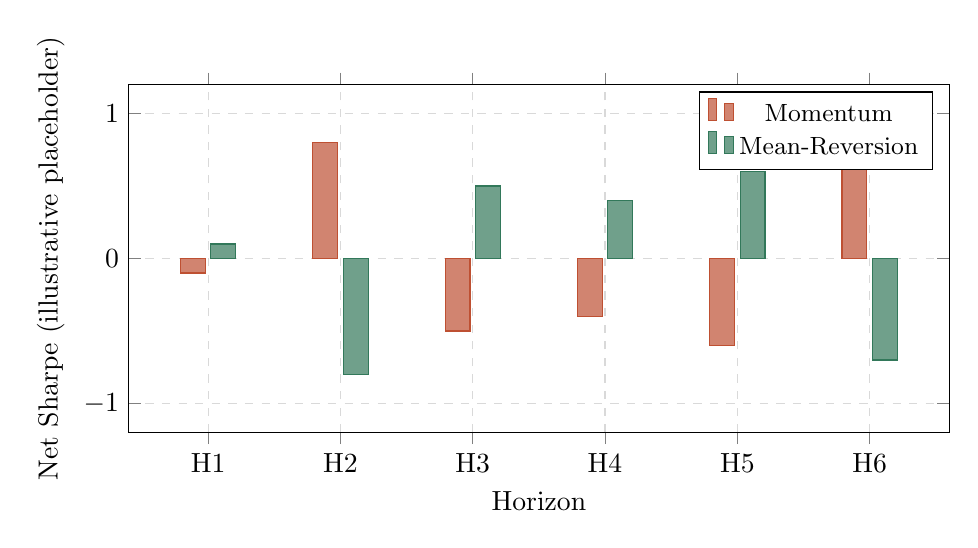
\begin{tikzpicture}
\begin{axis}[
  width=12cm, height=6cm,
  ybar,
  bar width=9pt,
  xtick=data,
  symbolic x coords={H1,H2,H3,H4,H5,H6},
  enlarge x limits=0.12,
  ylabel={Net Sharpe (illustrative placeholder)},
  xlabel={Horizon},
  ymin=-1.2, ymax=1.2,
  legend style={at={(0.98,0.98)},anchor=north east,font=\small},
  grid=major,
  grid style={dashed,gray!30}
]
\addplot[fill=momcol!70, draw=momcol] coordinates
 {(H1,-0.1) (H2,0.8) (H3,-0.5) (H4,-0.4) (H5,-0.6) (H6,0.7)};
\addplot[fill=meanrev!70, draw=meanrev] coordinates
 {(H1,0.1) (H2,-0.8) (H3,0.5) (H4,0.4) (H5,0.6) (H6,-0.7)};
\legend{Momentum, Mean-Reversion}
\end{axis}
\end{tikzpicture}
\caption{Illustrative outcome (numbers to be replaced by real estimates). The plot shows the net Sharpe of each strategy at each horizon. A clean sign-flipping pattern across horizons is the visual story.}
\label{fig:headline}
\end{figure}

\subsection{How we pick the two strategies for the ICM}

Let $h^*_{\text{MOM}} = \arg\max_h \text{SR}^{\text{MOM}}_h$ (subject to $t>t^*$) and similarly $h^*_{\text{REV}} = \arg\max_h \text{SR}^{\text{REV}}_h$. The ICM presents exactly these two strategies. If only one passes the significance threshold, we still present the best of each family but note the absence of significance.

%=================================================================
\section{Robustness and Statistical Checks}\label{sec:robust}
%=================================================================

The headline is the table. These checks travel alongside it in the ICM appendix.

\subsection{Variance ratio across horizons}

For each DJ30 name, compute the Lo--MacKinlay (1988) variance ratio
\begin{equation}
\VR(q) = \frac{\Var(r_{t,q})/q}{\Var(r_{t,1})} = 1 + 2\sum_{k=1}^{q-1}\Bigl(1-\tfrac{k}{q}\Bigr)\rho_k
\end{equation}
for $q\in\{2,5,21,126,252\}$ days, using CRSP. Pool across the 30 names for power. $\VR<1$ is the reversal signature; $\VR>1$ is momentum. The VR curve is the continuous-horizon version of our table---it should \emph{corroborate} the strategy results.

\subsection{One ML benchmark (single horizon)}

At the winning mean-reversion horizon, re-run the strategy with signals from a gradient-boosted-tree (LightGBM) regression on a modest feature set: past-return at several lags, trailing volatility, Amihud illiquidity from \texttt{iid\_ms}. Training: purged walk-forward on $T-1$ folds. Report whether the ML-enhanced Sharpe exceeds the naive-rank Sharpe by more than 1 standard error, using the Diebold--Mariano or Politis--Romano block bootstrap. If it does not, we conclude that naive ranking captures the available predictability and no ML uplift is warranted.

\subsection{Regime split}

For the two selected strategies, report net Sharpe within each of four VIX quintiles (pooled lowest two = calm; highest = crisis). This is reported once; it is not a trading rule.

\subsection{Cost sensitivity}

Report the break-even cost: the per-side $c_h$ at which the net Sharpe drops to zero. If break-even is below 1~bp, the strategy is not tradeable; if above 5~bp, the conclusion is robust.

\subsection{Survivorship and bias checks}

\begin{itemize}[leftmargin=*]
  \item Re-run using only always-present DJ30 members; confirm the direction of the bias (survivorship typically inflates gross momentum Sharpe; should attenuate under point-in-time).
  \item Verify no look-ahead: shift every feature by one additional day and rerun; Sharpe should drop only modestly if the strategy is genuinely ex-ante.
  \item Recompute returns using CRSP total returns (\texttt{ret}) rather than price-only (\texttt{retx}); material differences flag a dividend-handling bug.
\end{itemize}

%=================================================================
\section{ICM Deliverable}\label{sec:icm}
%=================================================================

\subsection{Structure}

A single ICM, roughly 20--25 pages, with these sections:

\begin{enumerate}[leftmargin=*,label=\arabic*.]
  \item \textbf{Executive Summary} (1 page): the two chosen strategies, headline Sharpe, headline risk, and recommendation.
  \item \textbf{Research Frame} (1 page): the horizon-comparison thesis, with Figure~\ref{fig:hypothesis}.
  \item \textbf{Methodology} (2 pages): universe, signal, portfolio construction, cost model---the unified specification.
  \item \textbf{The Horizon Comparison} (3 pages): Table~\ref{tab:headline}, Figure~\ref{fig:headline}, one paragraph of interpretation per horizon.
  \item \textbf{Selected Strategy \#1: ``Best Mean-Reversion''} (3--4 pages): detailed spec, equity curve, drawdown, factor regression, regime tables, profit/loss conditions.
  \item \textbf{Selected Strategy \#2: ``Best Momentum''} (3--4 pages): same format.
  \item \textbf{Statistical Properties} (2 pages): return distribution, autocorrelation, VaR/ES.
  \item \textbf{Robustness} (2 pages): VR curve, ML benchmark, regime split, cost sensitivity.
  \item \textbf{Implementation \& Risk} (1 page): capacity at realistic AUM, kill-switch rules.
  \item \textbf{Limitations} (1 page): DJ30 is a small cross-section; large caps attenuate classical effects; 10 years is a modest sample for H6.
  \item \textbf{Appendix} (as needed): code scaffolding, feature list, LLM log index, references.
\end{enumerate}

\subsection{Tone}

Sell-side memo style: short sentences, numbers in tables, no hedging without quantification. Replace ``the strategy performs well'' with ``gross SR 0.87, net SR 0.52, MDD 11\%.''

%=================================================================
\section{Week-by-Week Plan}\label{sec:plan}
%=================================================================

\begin{table}[H]
\centering
\small
\begin{tabularx}{\linewidth}{@{}l X@{}}
\toprule
\textbf{Week} & \textbf{Deliverable}\\
\midrule
1 & CRSP + \texttt{iid\_ms} loaders; point-in-time DJ30 universe built; daily panel merged.\\
2 & H3, H4, H5, H6 signals computed on CRSP; naive terciles backtested; cost model applied.\\
3 & H2 signal from \texttt{iid\_ms} (or TAQ if AM/PM not in IID); backtested; Gao regression reproduced.\\
4 & H1 from TAQ \emph{or} skip and document; full comparison table and headline figure drafted.\\
5 & Robustness suite: VR curve, regime split, cost sensitivity, single ML benchmark.\\
6 & ICM draft; peer review; revise.\\
7 & Polish, reproducibility (single \texttt{make all}), attribution log completed, submit.\\
\bottomrule
\end{tabularx}
\end{table}

%=================================================================
\section{Pitfalls}\label{sec:pitfalls}
%=================================================================

The short list; each has bitten similar studies before.

\begin{enumerate}[leftmargin=*]
  \item \textbf{Survivorship}: use point-in-time DJ30 membership, never today's 30.
  \item \textbf{Look-ahead}: all signals use information strictly at or before time $t$; \texttt{iid\_ms} is end-of-day, so use it at the \emph{next} session.
  \item \textbf{Corporate actions}: use CRSP \texttt{ret} (total return), not \texttt{retx}, and adjust prices by \texttt{cfacpr}. The DD $\to$ DWDP $\to$ DOW sequence in 2017--2019 is a known edge case.
  \item \textbf{Overlapping forecasts at H6}: 126-day holding periods overlap; naive $t$-stats overstate significance. Use non-overlapping monthly rebalances or Newey--West with $q=6$ lags.
  \item \textbf{In-sample scaling}: any feature normalization at H-ML benchmark must be fit on training folds only.
  \item \textbf{Turnover drift at H1}: 30-min rebalancing with ter\-cile flips generates large turnover; cost sensitivity is critical here.
  \item \textbf{Earnings days}: individual stocks have idiosyncratic jumps on earnings dates; document whether results are robust to excluding an earnings blackout window.
\end{enumerate}

%=================================================================
\section{LLM Usage and Attribution}\label{sec:attribution}
%=================================================================

Attribution is the easiest 25 of the 100 points. Maintain a numbered \texttt{llm\_logs/} directory with one file per non-trivial LLM interaction. Each entry records: model, date, prompt verbatim, output (or pointer), and how the output was used. The ICM appendix lists all entries by number with a one-line purpose. When in doubt, log it; under-reporting is penalized, over-reporting is not.

\begin{lstlisting}[basicstyle=\ttfamily\footnotesize]
[LLM-Log 012]
Model:     Claude Opus 4.7
Date:      2026-04-20 10:15 EDT
Prompt:    "Derive the closed-form Bonferroni threshold for 12 tests
            at family-wise alpha = 5%; explain the intuition."
Output:    [full in /llm_logs/012.txt]
Used for:  Section 4.7 of guide; confirmed threshold t* ~ 2.87.
\end{lstlisting}

%=================================================================
\section{Minimal Code Skeleton}\label{sec:code}
%=================================================================

A single, horizon-agnostic backtest loop keeps the comparison clean.

\begin{lstlisting}[language=Python]
import numpy as np, pandas as pd

def terciles_longshort(df, signal_col):
    """Return dollar-neutral equal-weight tercile long-short weights."""
    out = df.copy()
    out['rk'] = out.groupby('date')[signal_col].rank(method='first')
    out['n']  = out.groupby('date')['rk'].transform('size')
    out['q']  = pd.cut(out['rk']/out['n'],
                       bins=[0,1/3,2/3,1], labels=['lo','mi','hi'])
    w = np.where(out['q']=='hi',  1.0,
        np.where(out['q']=='lo', -1.0, 0.0))
    leg_size = out.groupby(['date','q'])['rk'].transform('size')
    w = w / leg_size
    out['w_mom'] = w
    out['w_rev'] = -w
    return out

def run_horizon(panel, h, cost_bps=1.5, target='ret_fwd'):
    """panel: long df with (date, permno, signal, ret_fwd). Returns P&L per rebalance."""
    p = terciles_longshort(panel, 'signal')
    pnl_mom_gross = (p['w_mom'] * p[target]).groupby(p['date']).sum()
    pnl_rev_gross = (p['w_rev'] * p[target]).groupby(p['date']).sum()
    turn = p.groupby('date').apply(lambda g: g['w_mom'].abs().sum())
    cost = turn * (cost_bps/1e4)
    return pd.DataFrame({
        'mom_gross': pnl_mom_gross,
        'mom_net':   pnl_mom_gross - cost,
        'rev_gross': pnl_rev_gross,
        'rev_net':   pnl_rev_gross - cost,
    })

def summarize(pnl, periods_per_year):
    def stats(x):
        mu, sd = x.mean(), x.std()
        sr = np.sqrt(periods_per_year) * mu / sd if sd > 0 else np.nan
        t  = np.sqrt(len(x)) * mu / sd if sd > 0 else np.nan
        return pd.Series({'mean': mu, 'std': sd, 'SR': sr, 't': t})
    return pnl.apply(stats).T
\end{lstlisting}

The same \texttt{run\_horizon} is called six times with six different $(h, \text{signal}, \text{target})$ triples; the summary table is the concatenation.

%=================================================================
\section{Selected References}\label{sec:refs}
%=================================================================

\begin{description}[leftmargin=0cm, itemsep=0.2em]
\item[DeBondt \& Thaler (1985)] Does the Stock Market Overreact? \textit{J.~Finance.}
\item[Fama \& French (1988)] Permanent and Temporary Components of Stock Prices. \textit{JPE.}
\item[Gao, Han, Li, Zhou (2018)] Market Intraday Momentum. \textit{JFE.}
\item[Jegadeesh (1990)] Evidence of Predictable Behavior of Security Returns. \textit{J.~Finance.}
\item[Jegadeesh \& Titman (1993)] Returns to Buying Winners and Selling Losers. \textit{J.~Finance.}
\item[Lehmann (1990)] Fads, Martingales, and Market Efficiency. \textit{QJE.}
\item[Lo (2004)] The Adaptive Markets Hypothesis. \textit{JPM.}
\item[Lo \& MacKinlay (1988)] Stock Market Prices Do Not Follow Random Walks. \textit{RFS.}
\item[Lo \& MacKinlay (1990)] When Are Contrarian Profits Due to Stock Market Overreaction? \textit{RFS.}
\item[Moskowitz \& Grinblatt (1999)] Do Industries Explain Momentum? \textit{J.~Finance.}
\item[Nagel (2012)] Evaporating Liquidity. \textit{RFS.}
\item[Politis \& Romano (1994)] The Stationary Bootstrap. \textit{JASA.}
\item[Roll (1984)] A Simple Implicit Measure of the Effective Bid-Ask Spread. \textit{J.~Finance.}
\end{description}

\bigskip
\begin{center}
\itshape Guide v3 --- lean \& comparison-centric. The headline is Table~\ref{tab:headline}.
\end{center}

\end{document}